Una de las mayores causas de accidentes son las distracciones de los conductores
al volante, o bien por el uso de dispositivos electrónicos, somnolencia u otras
acciones que llevan a la persona a no prestar atención a la carretera y su entorno.

A raíz de ese problema, los mecanismos de regulación internacionales han invertido
tiempo, dinero y desarrollo en los sistemas ADAS (\textit{Advanced Driving Assistance Systems}),
con el fin de mitigar las situaciones anteriores y realizar una prevención activa
sobre los accidentes de tráfico. Sin embargo, dichos sistemas no cuentan con una
penetración significativa en el mercado, por lo que interesa agilizar su implantación
y que pasen a ser un elemento de seguridad ``por defecto'' en los nuevos vehículos.

En este contexto, se ha pedido realizar una implementación distribuida, que cumpla con
unos requisitos de tiempo real, en dos nodos que interactúan entre sí para actuar
como un organismo conjunto sobre un vehículo como sistema ADAS.

El sistema a desarrollar contará con múltiples sensores:
\begin{itemize}
  \item Giroscopio, para detectar en los ejes $X$ y $Y$ la inclinación de la cabeza
        del conductor y predecir una posible somnolencia.
  \item Giro del volante, para detectar si el conductor está pegando volantazos o está
        realizando ``mini--correcciones'', características de un estado de somnolencia o
        de atender al móvil.
  \item Agarre del volante, donde se indicará si el conductor está agarrando el volante
        o no.
  \item Velocímetro, con un rango de valores comprendido entre los
        $\left[0, 200\right] \nicefrac{km}{h}$. Se usará para comprobar que se cumple
        la distancia de seguridad.
  \item Sensor de distancia, capaz de realizar lecturas en el rango $\left[5, 200\right]~m$
        y que le indicará al conductor si está cumpliendo o no la distancia de seguridad,
        según la velocidad a la que circule.
\end{itemize}

y múltiples actuadores:
\begin{itemize}
  \item Luces de aviso, las cuales se usarán para emitir señales luminosas al conductor
        indicando cierto nivel de riesgo que se está produciendo.
  \item \textit{Display}, usado para visualizar los datos que obtiene el sistema.
  \item Alarma sonora, emitiendo un sonido con 3 niveles de intensidad.
  \item Luz de aviso/freno automático, donde ante un peligro de colisión inminente
        el sistema podrá activar el freno con hasta 3 niveles de intensidad.
\end{itemize}

Cada uno de los sensores/actuadores estarán controlados y monitorizados por una o
varias tareas las cuales registran los datos en objectos protegidos. Dichas tareas
vienen definidas con sus periodos y \textit{deadlines} en el cuadro \ref{tab:tasks}:

\begin{table}[H]
  \centering
  \begin{tabularx}{\linewidth}{C{.3}|c|c|c|c|c|c|c}
    \textbf{Tareas/objetos protegidos} & \textbf{Tipo} & $T_i$  & $D_i$  & \textbf{WCET} & \textbf{Síntomas 1} & \textbf{Síntomas 2} & \textbf{Modo} \\
    \hline
    Inclinación cabeza                 & C             & $600$  & $400$  & ?             & $x_1$               &                     &               \\
    Detección de volantazos            & C             & $400$  & $400$  & ?             & $x_1$               &                     &               \\
    Cálculo distancia                  & C             & $300$  & $300$  & ?             &                     & $y_1$               &               \\
    Relax al volante                   & C             & $500$  & $200$  & ?             & $x_1$               &                     &               \\
    Emergencias                        & C             & $300$  & $300$  & ?             & $x_2$               & $y_2$               & $z_2$         \\
    Mostrar información                & C             & $2000$ & $2000$ & ?             & $x_2$               & $y_2$               &               \\
    Detección pulsador                 & S             & -      & $100$  & ?             &                     &                     & $z_1$         \\
    \hline\hline
    Síntomas 1                         & P             & -      & -      & $x_1, x_2$    &                     &                     &               \\
    Síntomas 2                         & P             & -      & -      & $y_1, y_2$    &                     &                     &               \\
    Modo                               & P             & -      & -      & $z_1, z_2$    &                     &                     &               \\
    \hline\hline
  \end{tabularx}
  \caption{Listado de tareas y objetos protegidos junto con sus tiempos.}
  \label{tab:tasks}
\end{table}

Como hay multitud de tareas y se cuenta con dos nodos, el sistema a implementar irá
distribuído entre ambos y viene representado por la figura \ref{fig:system-full}:

\begin{figure}[H]
  \centering
  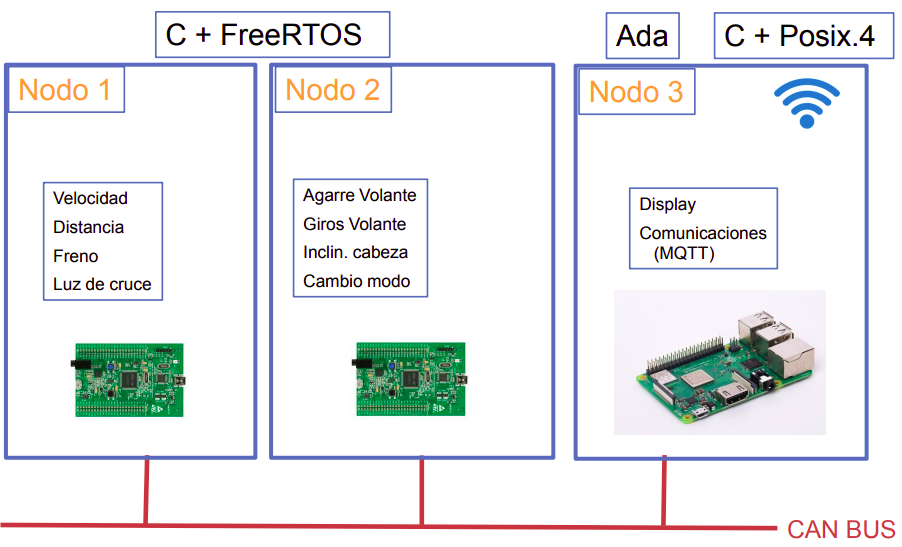
\includegraphics[width=.7\linewidth]{pictures/system-full.png}
  \caption{Modelo completo del sistema a implementar. Las tareas van distribuídas entre
    los dos nodos principales y se comunican entre ellos mediante CANBus.}
  \label{fig:system-full}
\end{figure}